\documentclass[12pt]{article}

\usepackage{scicite,times,graphicx,float,hyperref}
\usepackage[skip=0pt]{caption}
\usepackage[utf8]{inputenc}
\usepackage{enumitem}
\usepackage{booktabs}

\topmargin -1.0cm
\oddsidemargin 0.0cm
\textwidth 16cm 
\textheight 23cm
\footskip 1.0cm

\newenvironment{sciabstract}{%
\begin{quote} \bf}
{\end{quote}}

\newcounter{lastnote}
\newenvironment{scilastnote}{%
  \setcounter{lastnote}{\value{enumiv}}%
  \addtocounter{lastnote}{+1}%
  \begin{list}%
  {\arabic{lastnote}.}
  {\setlength{\leftmargin}{.22in}}
  {\setlength{\labelsep}{.5em}}
}
{\end{list}}

\title{A Farm Simulation\\using Swing and Concurrency} 

\author
{Filipe Pires [85122], João Alegria [85048]\\
\\
Software Architecture\\
\normalsize{Department of Electronics, Telecommunications and Informatics}\\
\normalsize{University of Aveiro}\\
} 

\date{\today{}}

%%%%%%%%%%%%%%%%% END OF PREAMBLE %%%%%%%%%%%%%%%%

\begin{document} 

\baselineskip18pt

\maketitle 

\section{Introduction} %%%%%%%%%%%%%%%%%%%%%%%%%%%%%%%%%%%%%%%%%%%%%%%%%%%%%%%%%%%%%%%%%%%%%%%%%%%%%%%%%%%%%%%%%%%%%%%%%%%%%%%%%%%%%%%%%%%%%%%%%%%%%%%%%%%%%%%%%

This report aims to describe the work developed for the first assignment of the course of 'Software Architecture', explaining the overall architecture and 
describing its components and respective communication channels and elaborating on the adopted solutions for concurrency.
We also mention how the work was distributed amongst the authors.

The Java application has the purpose of conducting harvest simulations on an agricultural farm.
Along with the technical aspects of the implementation, we also elaborate on the adopted solutions for concurrency.
Efforts on making the UI highly usable and the code readable and well documented are also stated here.
All code developed is publicly accessible in our GitHub repository:
\url{https://github.com/FilipePires98/AS/}.
\newpage

\section{The Agricultural Farm} \label{farm} %%%%%%%%%%%%%%%%%%%%%%%%%%%%%%%%%%%%%%%%%%%%%%%%%%%%%%%%%%%%%%%%%%%%%%%%%%%%%%%%%%%%%%%%%%%%%%%%%%%%%%%%%%%%%%%%%%%

Agricultural farms have well defined seasons where different activities must be executed to maintain the business productive.
Tasks must be distributed amongst workers and quantities must be calculated and tracked for the correct functioning of the entire farm.
As the whole system grows, its complexity and difficulty in management grows as well, so management tools emerge as valuable assets for farmers.

Amongst the many features of such tools, one offers a particularly interesting view of the farm as it simulates its behavior.
Such simulations allow farm owners to plan harvests and test strategies to understand which offer the greatest productivity and profit.
These simulator tools may be as complex as the farm itself, but allow manipulation of time and other resources without any cost.
So, it is easy to understand that solutions of this nature offer value to the farming audience in general.

With this in mind, it was proposed to us to develop an agricultural farm harvest simulator with very simple features in order to apply the knowledge gained 
during the course.
This simulator isn't meant to serve as a final product for an agricultural business, rather it should show the potential of such solutions.
As it implements concurrency by design, it ensures scalability for a potential product and offers realistic aspects on the virtual farmers' behavior.

But how exactly is the system organized?
There are two main entities: the Control Center (CC) and the Farm Infrastructure (FI). 
The CC is responsible for supervising the harvest, while the FI is the infrastructure for the agricultural harvest.

\subsection{Control Center} %%%%%%%%%%%%%%%%%%%%%%%%%%%%%%%%%%%%%%%%%%%%%%%%%%%%%%%%%%%%%%

The Control Center is where the number of farmers out of the 5 should be selected to participate in the harvest run is defined, along with their maximum step size, the amount of corn cobs each farmer should collect and a special parameter called timeout.
Timeout, defined in milliseconds, is a parameter used for regulation of the simulation's execution time and sets the time interval each farmer should take to make a movement.

It is in the CC that users send orders for the virtual farmers to execute.
The commands available are:
\vspace{-10pt}
\begin{itemize}[noitemsep]
  \item Prepare - the selected farmers move to a Standing Area, ready for orders.
  \item Start - the actual simulation begins and farmers start moving.
  \item Collect - farmers collect corn cobs from the Granary (where the cobs initially are).
  \item Return - farmers return to the Storehouse with the collected corn cobs.
  \item Stop - farmers stop whatever they are doing and return to the Storehouse.
  \item Exit - simulation ends and the program closes.
\end{itemize}
\vspace{-10pt}

\subsection{Farm Infrastructure} %%%%%%%%%%%%%%%%%%%%%%%%%%%%%%%%%%%%%%%%%%%%%%%%%%%%%%%%%

The Farm Infrastructure is the part of the system that has the virtual components of the farm.
It holds four sections of the farm:
\vspace{-10pt}
\begin{itemize}[noitemsep]
  \item Storehouse - where farmers rest and corn cobs are stored.
  \item Standing Area - where selected farmers wait for further orders.
  \item Path - a representation of the field that farmers must cross.
  \item Granary - where corn cobs are temporarily stored.
\end{itemize}
\vspace{-10pt}
FI also supports virtual farmers, which during their lives transit between the following states:
\vspace{-10pt}
\begin{itemize}[noitemsep]
  \item Initial - resting (blocked) in the Storehouse.
  \item Prepare - ready for orders (blocked) in the Standing Area.
  \item Walk - moving in the Path (one by one, in the same order they entered it) towards the Granary.
  \item Wait to Collect - waiting for orders (blocked) to collect corn cobs in the Granary.
  \item Collect - collecting corn cobs from the Granary.
  \item Return - moving in the Path (one by one, in the same order they entered it) towards the Storehouse, with the collected cobs.
  \item Store - storing the collected corn cobs in the Storehouse.
  \item Exit - farmer kills itself.
\end{itemize}
\vspace{-10pt}
So, as you can see, there is a direct mapping between the commands made available to users and the farmer states.
\newline 

When deployed, the system offers a Graphical User Interface (GUI) for each entity.
CC's UI allows user interaction and FI's UI allows visualization of the simulation in real time.
We added to CC's interface a mirror of FI's to allow the possibility of both entities running in different environments far away from each other, while ensuring 
that the user on CC's side has knowledge of what is happening during the simulation.
This and other interface-related aspects will be mentioned in greater detail further ahead.

\begin{figure}[H]
  \centering
  \begin{minipage}{\textwidth}
    \centering
    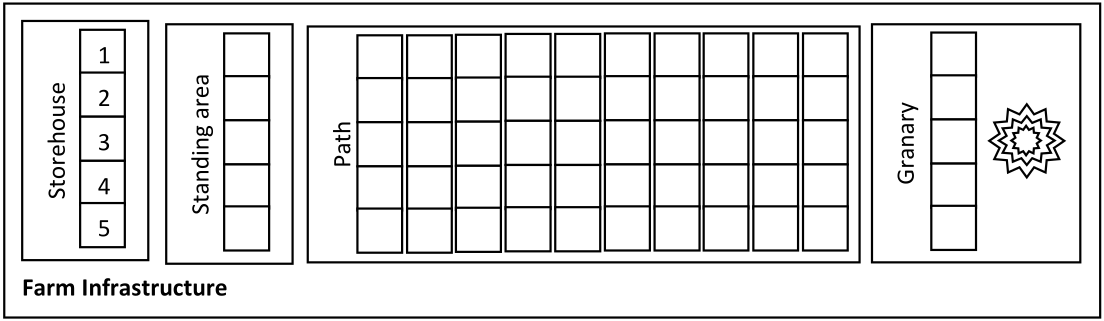
\includegraphics[width=\linewidth]{img/Design_FI.png}
  \end{minipage}%
  \caption{Visual representation of the farm, taken from \cite{assign}.}
  \label{Design_FI}
\end{figure} 

\newpage
\section{System Architecture} %%%%%%%%%%%%%%%%%%%%%%%%%%%%%%%%%%%%%%%%%%%%%%%%%%%%%%%%%%%%%%%%%%%%%%%%%%%%%%%%%%%%%%%%%%%%%%%%%%%%%%%%%%%%%%%%%%%%%%%%%%%%%%%%%%

In this chapter we focus on the implementation of each component and on the architecture of the entire solution.
Here, we resort to a class diagram (see Figure \ref{ClassDiagram}) in UML \cite{uml} to visually aid interpretation.
We also present screenshots of the GUIs to explain how the interaction works.

Our harvest simulator follows a modular structure implemented in Java.
As we will see, each component has a specific purpose and is responsible for one key aspect of the system's functionality.
The principle of least knowledge is here applied and code dependency is kept low.
This means that there are no unnecessary elements but it is needless to say that without any of the components the system will not work as intended.

Components belonging to the same logical layer are grouped within a package.
Communications between independent components are done through defined protocols. 
The system is designed to be extensible as well, through the use of well defined interfaces that allow the creation of new versions of farm areas without 
refactoring the main entities.

All relevant actions during simulations are printed to a unique terminal, with the due source identification, allowing an easy management of what is occurring 
during execution.
To deal with exceptions thrown by user commands, we designed our own exception handling mechanisms.
Also, since the user side is the greatest potential source of errors, the interface is confined to its most limited usage, i.e. users are only allowed to do 
what they can actually do at all times.
Although this may seem to reduce the usability of the solution, it actually helps users by guiding them towards what they want to do, without leaving margin for errors.

\subsection{Components} %%%%%%%%%%%%%%%%%%%%%%%%%%%%%%%%%%%%%%%%%%%%%%%%%%%%%%%%%%%%%%

Once the Java application is executed, out Main class launches a subprocess dedicated to the FarmInfrastructure and instantiates the ControlCenter, passing full 
control to it.
Every Java application has a single instance of class java.lang.Runtime that allows the application to interact with the environment in which it is running.
By obtaining the environment through \textit{Runtime.getRuntime()} and calling the \textit{Runtime.exec(String command)} method, the Main class is able to launch 
an independent Java process and manage it - allowing the existance of the previously mentioned unique terminal for printing system status during runtime.
The \texttt{command} string is built by retrieving the directory where the code is located:  

\texttt{java -cp <userdir>/build/classes fi.FarmInfrastructure}

\begin{figure}[H]
  \centering
  \begin{minipage}{1.05\textwidth}
    \centering
    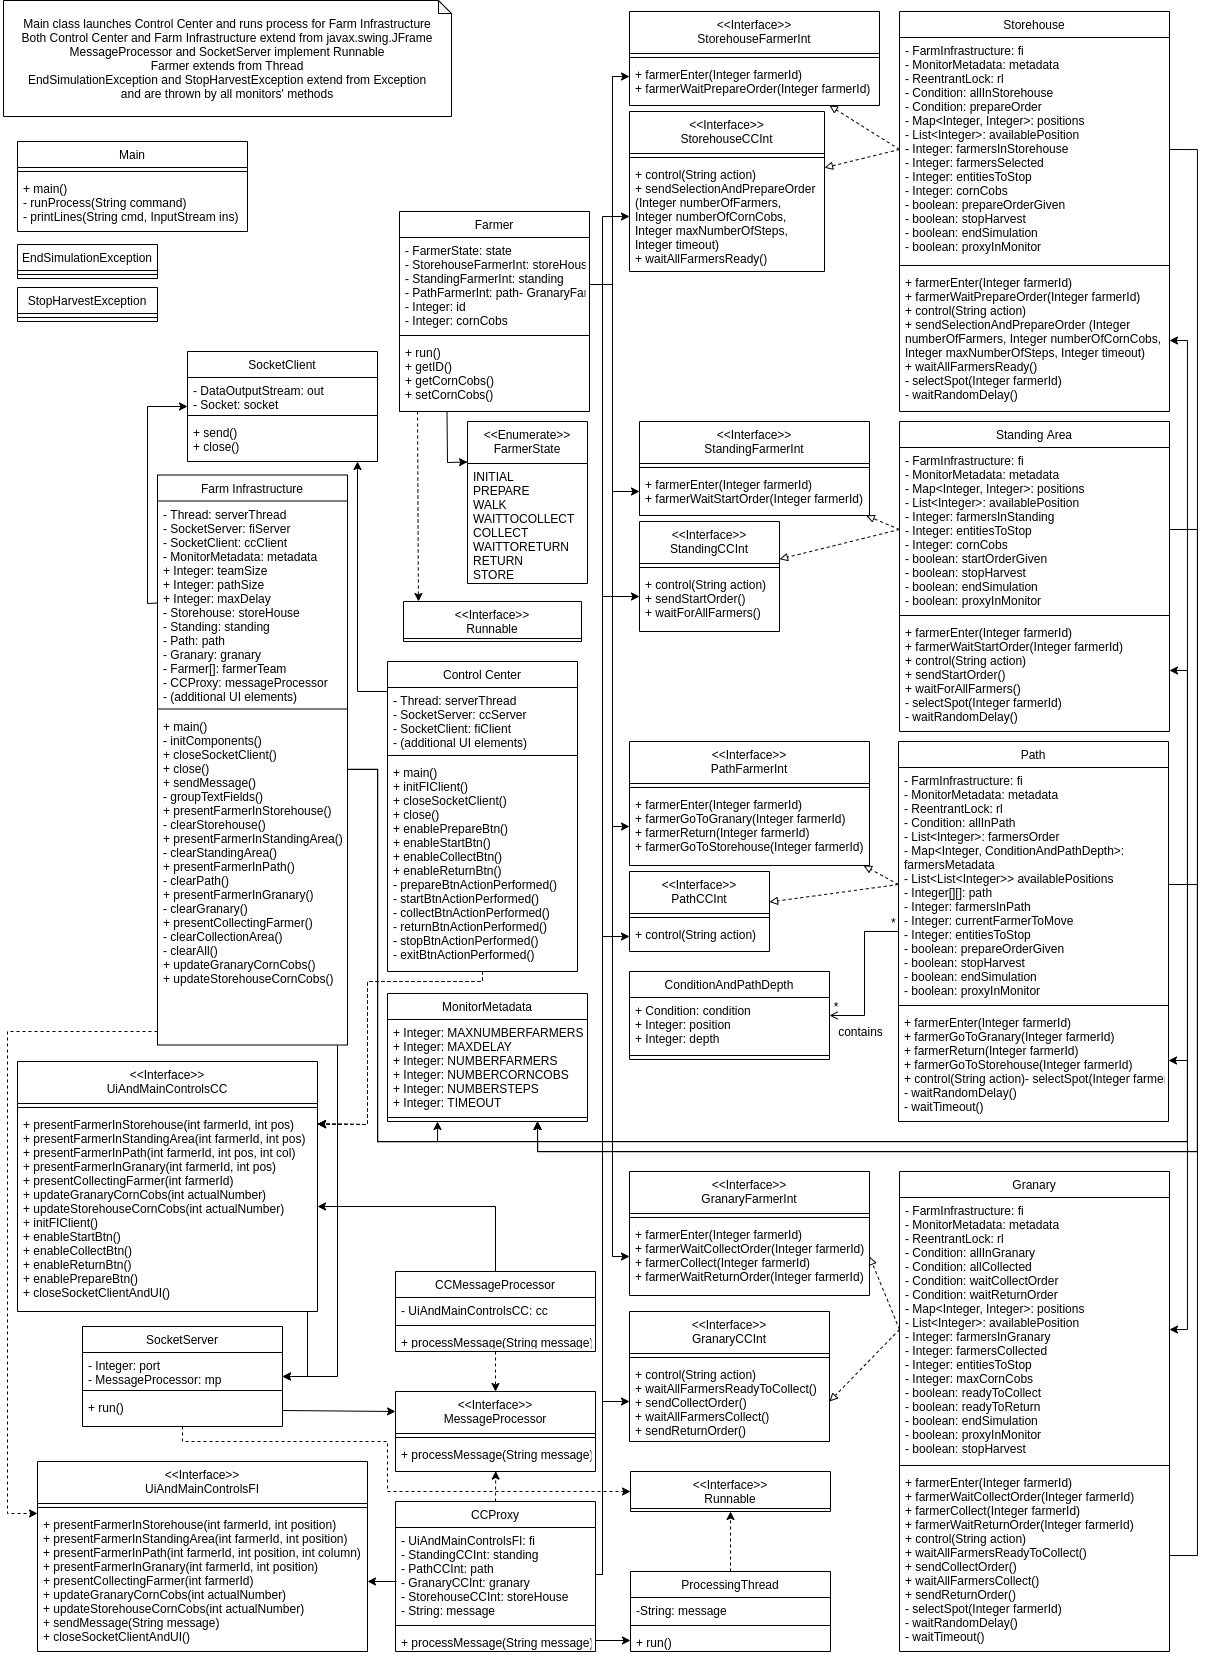
\includegraphics[width=\linewidth]{img/ClassDiagram.png}
  \end{minipage}%
  \caption{Class diagram of the Farm Simulation application.}
  \label{ClassDiagram}
\end{figure} 

Now we have our two entities - the system's core.
ControlCenter and FarmInfrastructure implement the UiAndMainControlsCC interface and UiAndMainControlsFI interface respectively.
Both classes extend from \texttt{javax.swing.JFrame} and contain the code regarding the GUIs and communicate with each other with the use of sockets.
Both have instances of SocketServer and SocketClient, that in return have instances of \texttt{java.net.Socket}, and together establish a two-way communication channel.
Communication establishment is explained in section \ref{communications}.

Farmers are simulated as thread instances from the same class.
Their states are defined in the FarmerState enumerate.
When instantiated by FI, they enter the Storehouse and wait for further orders that will guide their lifecycle of retrieving and storing virtual corn cobs.
MonitorMetadata, as the name states, contains the metadata of the monitors (the farm areas).
This information applies constraints to the farm areas where farmers will pass, hence influencing the execution flow according to the users' wishes.
As each farmer has its own execution thread, their access to shared resources must be controlled.
This is where the monitors come in hand. 
The concurrency measures implemented by our monitors are justified in section \ref{monitors}. 

\subsection{User Interface} %%%%%%%%%%%%%%%%%%%%%%%%%%%%%%%%%%%%%%%%%%%%%%%%%%%%%%%%%

Having succinctly gone through all components, we move on to presenting the user interface and explaining its confinements.
Built with Swing \cite{swing}, the UIs remain faithful to the design concept proposed for the simulation, with some improvements.

In Figure \ref{UserInterface_FI} we see a screen capture during runtime of the FI interface.
Here, the user holds no control and only sees what is happening to each Farmer thread by tracking the movement of their IDs.
Note that the IDs correspond to internal class identifiers and not the actual thread identifiers.
This means that, if desired, such IDs could be replaced by strings containing the farmer names for example (as long as they were unique, of course).

\begin{figure}[H]
  \centering
  \begin{minipage}{.9\textwidth}
    \centering
    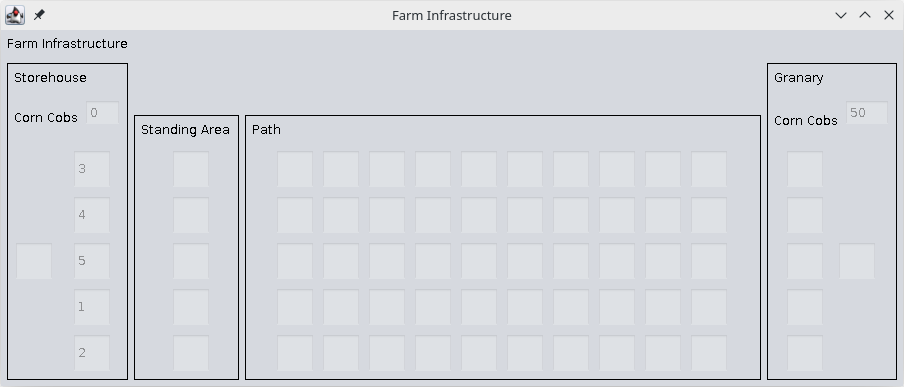
\includegraphics[width=\linewidth]{img/UserInterface_FI.png}
  \end{minipage}%
  \caption{Screenshot of the FI UI.}
  \label{UserInterface_FI}
\end{figure} 

Now Figures \ref{UserInterface_CC_1}, \ref{UserInterface_CC_2} and \ref{UserInterface_CC_3} offer a more interesting view on the system.
Just by looking at them a few conclusions can be drawn relevant to our situation.
First of all, with all farmers launched and ready in the Storehouse, only the usable buttons are enabled.
At this stage the user is allowed to define the parameters on the controls panel on the bottom.
Such controls are well labelled and use spinners for defining integer values in order to avoid user errors.

\vspace{-5pt}
\begin{figure}[H]
  \centering
  \begin{minipage}{.9\textwidth}
    \centering
    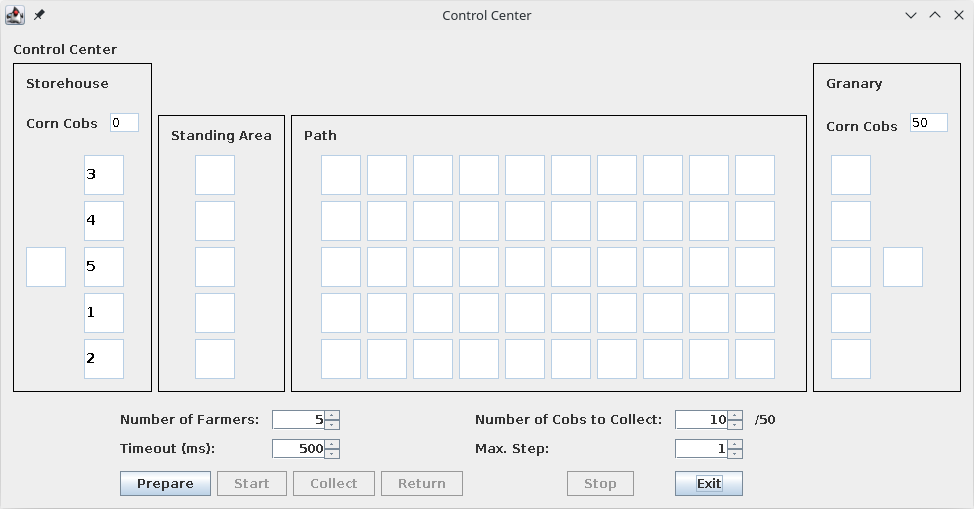
\includegraphics[width=\linewidth]{img/UserInterface_CC_1.png}
  \end{minipage}%
  \caption{Screenshot of the CC UI right after launching the application.}
  \label{UserInterface_CC_1}
\end{figure}
\vspace{-10pt}

When we look at Figure \ref{UserInterface_CC_2}, we see that CC is capable of following the simulation just like FI.
By comparing such figure with \ref{UserInterface_CC_3} we also understand that each button is only enabled when the selected farmers are all ready to 
comply with such commands (see the 'Collect' button).
The requirement of randomness during path walking can also be inferred through Figure \ref{UserInterface_CC_2}, as farmers do not walk always in the same line 
nor at the same speed.

\vspace{-5pt}
\begin{figure}[H]
  \centering
  \begin{minipage}{.9\textwidth}
    \centering
    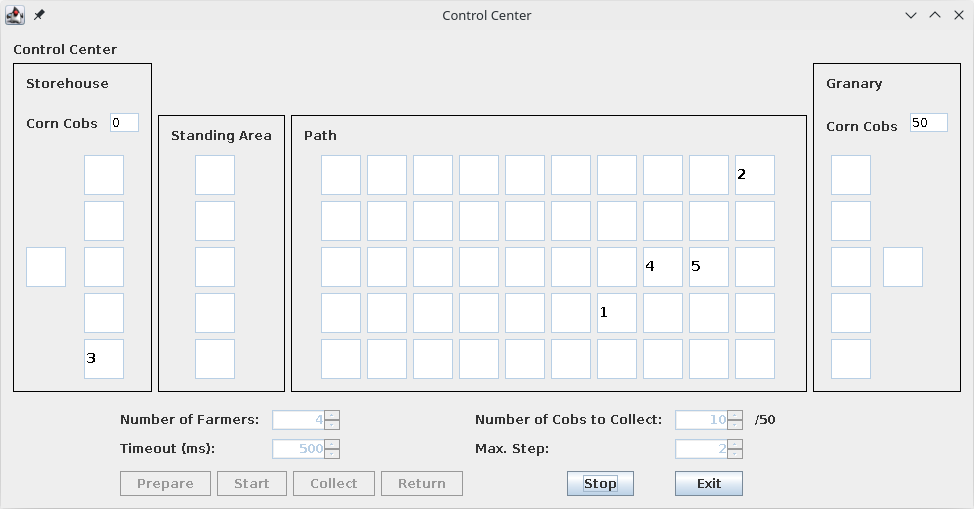
\includegraphics[width=\linewidth]{img/UserInterface_CC_2.png}
  \end{minipage}%
  \caption{Screenshot of the CC UI while farmers are crossing the Path.}
  \label{UserInterface_CC_2}
\end{figure} 
\vspace{-10pt}

\vspace{-10pt}
\begin{figure}[H]
  \centering
  \begin{minipage}{.9\textwidth}
    \centering
    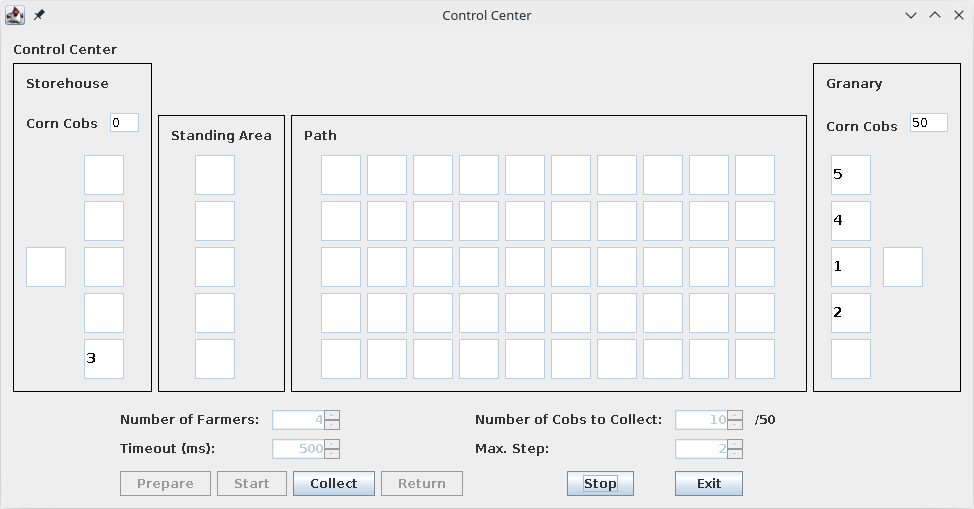
\includegraphics[width=\linewidth]{img/UserInterface_CC_3.png}
  \end{minipage}%
  \caption{Screenshot of the CC UI when the farmers are ready to collect corn cobs.}
  \label{UserInterface_CC_3}
\end{figure} 
\vspace{-10pt}

Two additional features are here worth mentioning.
The existence of a unique corn collecting position inside the Granary was already suggested in the initial design, however we decided this would also make sense
on the Storehouse as farmers would also store the corn cobs one at a time there.
Tracking the number of corn cobs was not a concern on the design concept, but we found it to be very important, even for debugging during development.
For this reason we also added small trackers both on the Storehouse and in the Granary that automatically update the number of cobs when it is changed.

The reason we decided to include a visual representation of the farm on the side of CC was that we considered the entities running on different and independent 
processes that could very well be running in different machines - with the only requirement of having knowledge of the endpoints and ports.
This meant that the Control Center should also have access to the state of the Farm Infrastructure and its components and workers or else it might not know 
if clicking the buttons was having any effect on the system.
In reality, what CC sees is a mirror of what FI presents, so there is an unnoticeable transmission delay.

\subsection{Interacting with the Infrastructure} %%%%%%%%%%%%%%%%%%%%%%%%%%%%%%%%%%%%

As the FarmInfrastructure must be in control of all that occurs during the harvest, this class instantiates and interacts with many elements.
Such interactions involve communicating with the ControlCenter, following the farmers and making available the farm areas.
For an easy analysis of this flow of events, orders and task executions, we designed an interaction diagram present in Figure \ref{InteractionDiagram}.
This diagram includes how the process starts and ends and what occurs in the event of exceptions.

\vspace{-10pt}
\begin{figure}[H]
  \centering
  \begin{minipage}{.9\textwidth}
    \centering
    \includegraphics[width=\linewidth]{img/InteractionDiagram.png}
  \end{minipage}%
  \caption{Interaction diagram of the Farm Infrastructure.}
  \label{InteractionDiagram}
\end{figure} 
\vspace{-10pt}

\newpage
\section{Concurrency Strategy} %%%%%%%%%%%%%%%%%%%%%%%%%%%%%%%%%%%%%%%%%%%%%%%%%%%%%%%%%%%%%%%%%%%%%%%%%%%%%%%%%%%%%%%%%%%%%%%%%%%%%%%%%%%%%%%%%%%%%%%%%%%%%%%%%

Implementing the system concurrent from the very core was essential to us, as it was required for farmers to "live" simultaneously while sharing resources and 
these resources (farm areas positions and corn cobs) would have to be managed in such way that data integrity was kept at all times.
Therefore, design decisions had to be made in order to deliver a robust and efficient solution.
Such concurrency strategies are here described and justified including: the synchronization methods applied to each farm area, the means of communication between
the main entities, and the exception handling solutions for user stop and shutdown orders.

\subsection{Monitors \& Farmers} \label{monitors} %%%%%%%%%%%%%%%%%%%%%%%

Amongst the four monitors of FI, only one was implemented using the implicit monitor lock accessed using synchronized methods.
The StandingArea is a monitor meant to ensure all selected threads are ready to follow orders.
Commands given are to be executed by all threads here locked and therefore this implicit lock mechanism was ideal.

Now, for all other monitors, synchronization wasn't as trivial.
As more than one condition should unlock specific threads at given moments, a more powerful synchronization mechanism was required.
And this is where Reentrant Locks come in.
A ReentrantLock \cite{reentrantlock} instance is a reentrant mutual exclusion lock with the same basic behavior and semantics as the implicit monitor lock, 
but with extended capabilities which include: the ability to have more than one condition variable per monitor; the ability to make the lock fair, unlike the 
implicit lock, i.e. a lock that favors granting access to the longest-waiting thread; the ability to check if the lock is being held; the ability to get the 
list of lock waiting threads.

Storehouse needed two conditions to know if all Farmer threads were ready to be used and if the command 'Prepare' had been given.
The Granary needed four to check if all selected farmers were inside the Granary to collect corn, to know if the commands 'Collect' and 'Return' had 
been given, and to check if all farmers had attempted to collect corn cobs.
The Path needed one condition to determine whether all selected farmers were in it or not, and a condition for each farmers walking the Path. The Path monitor was the one that really took advantage of the fact that we could create as many conditions inside an unique ReentrantLock as we wanted. We decided to create a condition for each farmers because it was important to us to maintain the solution scalable, and imagining a scenario where there were hundreds of farmers walking in thPath, it was not feasible to notify everyone when only one specific farmer needed to be notified. For that reason, with auxiliary data structures, we registered the order in which the farmers should walk in the path and created a condition to each one of them, making each farmer notify the next until all reached the end of the section.

Additional constraints implemented by these monitors are: at any given moment, only one farmer is inside a box; a random delay of up to 100ms is provided 
between each lock and the correspondent unlock.
These increase faithfulness to reality of the harvest simulation.

\subsection{Communications} \label{communications} %%%%%%%%%%%%%%%%%%%%%%%%%%%%%%%%%%

The adopted communication system was, as you might have guessed by now, messaging through sockets - as required \textit{a priori}. % using strings as messages. 
To do this, we implemented two auxiliary classes to enable both client (SocketClient) and server (SocketServer) sides, ready for usage. 
Each entity (CC and FI) has an instance of each of these classes, hence the reality of being both servers and clients.

Taking a closer look at the communication system's implemented and starting on the SocketClient, this class establishes a connection to the endpoint and port 
defined in its constructor.
Through its \textit{send(string message)} method, it is able to send requests to the socket server on the other end of the connection.
The \textit{close()} method, as the name implies, closes the socket connection previously established.

In relation to the SocketServer class, it implements a ready-to-use server deployed in the port provided in the constructor. 
It is implemented based on a thread, so that the server life-cycle can occur parallel to the main logic of the problem. 
The server is constantly waiting to receive a message, that when received is automatically passed to the MessageProcessor instance provided also in the constructor. 
The server dies only after receiving and processing a predefined message - the string "endSimulationOrder".

A SocketServer instance is provided with a MessageProcessor as the internal message processing logic.
MessageProcessor is an interface that any class containing message processing logic should implement and that requires the implementation of the method 
\textit{processMessage(string message)}. 
Each entity has a different implementation of MessageProcessor with the proper functionalities for the tasks required: CCMessageProcessor and CCProxy.
CCMessageProcessor is responsible for processing any messages the CC receives. 
This implementation processes the messages in a sequential form.
On the other hand, CCProxy acts as the message processor for those destined to the Farm Infrastructure as well as a substitute for the Control Center in the 
Farm Infrastructure process. 
Being a entity in a highly concurrent environment, a thread-based processing was implemented, meaning that for each received message, a new \texttt{Thread} was 
initiated with its life-cycle defined in the ProcessingThread class (a Runnable interface instance). 
This approach allows the correct handling of several messages simultaneously - a crucial aspect in the FI environment. 
The ProcessingThread class is the one containing the actual logic for the processing of each message the FarmInfrastructure receives.

Many of these classes and their interaction with FI are visible in the diagram of Figure \ref{InteractionDiagram}.
This section is also meant to elucidate such interactions.

\subsection{Exceptions} %%%%%%%%%%%%%%%%%%%%%%%%%%%%%%%%%%%%%%%%%%%%%%%%%%%%%%%%%%%%%%

When developing the solution for this complex concurrent scenario, the 'Stop Harvest' and 'End Simulation' events triggered by the user at any time were 
responsible for many of our doubts and difficulties.
Since farmer threads can be locked in quite different points of their life-cycle, a solution to notify them all that wouldn't imply verifying at each new step 
if such triggers had been activated was not natural nor immediate and needed to be found.

After many discussions and trials, the exception-handling approach was selected and implemented. 
Exceptions enabled us to only verify if the harvest stopping and simulation ended conditions were true in a few strategic places.
If one such condition was found to be true, the corresponding exception is thrown and the current thread executing the code automatically stops its current task 
and jumps to the exception catching code, enabling us to process that event. 
For this purpose, we create two custom exception classes, the StopHarvestSimulation and the EndSimulationException, both with self-explaining names.

\newpage
\section{Additional Remarks} %%%%%%%%%%%%%%%%%%%%%%%%%%%%%%%%%%%%%%%%%%%%%%%%%%%%%%%%%%%%%%%%%%%%%%%%%%%%%%%%%%%%%%%%%%%%%%%%%%%%%%%%%%%%%%%%%%%%%%%%%%%%%%%%%%%

\subsection{Documentation} %%%%%%%%%%%%%%%%%%%%%%%%%%%%%%%%%

Packages, interfaces, classes and methods are all documented, with the help of Javadoc \cite{javadoc}, and naming conventions are applied throughout the code, 
focusing on allowing readers to understand what methods do and variables are for by reading their names alone.

A significant effort was placed on this as we understood it would be greatly beneficial in the long term.
And it was indeed. As soon as one developer completed a component and ensured the textual guidance, the other would quickly be up-to-date on the internal 
functioning of such component in his own tasks.

Creating the diagrams here presented also allowed to keep a wider perspective on the project and discuss important issues during debugging while maintaining 
the same mental picture.

\subsection{Assignment Contributions} %%%%%%%%%%%%%%%%%%%%%%

Regarding the work distribution amongst developers, a close-contact strategy was defined where each worked on a piece of software according to a predefined plan. 
The project structure and architecture was decided in conjunction, as well as the key concurrency solutions chosen.
Both servers were also implemented collectively.

Nevertheless, some relatively independent task distribution was defined: João implemented the Granary and Path monitors, while Filipe did the Storehouse and 
Standing monitors; João established socket communications and respective message processors, while Filipe designed the user interface and respective interaction
with the remaining components.
Bug and error solving was made along the development phase by both developers any time it was required.

Once the final version of the application was completed, this report and the code documentation became our primary concern, with both contributing equally.

\newpage
\section{Conclusions} %%%%%%%%%%%%%%%%%%%%%%%%%%%%%%%%%%%%%%%%%%%%%%%%%%%%%%%%%%%%%%%%%%%%%%%%%%%%%%%%%%%%%%%%%%%%%%%%%%%%%%%%%%%%%%%%%%%%%%%%%%%%%%%%%%%%%%%%%%

After completing the assignment, we drew a few conclusions regarding the topics here explored and our endeavor to deliver work of quality.
First of all, it was quite interesting to learn more complete synchronization tools like the Reentrant Lock whose existence we weren't aware of.
Such mechanism allowed us to gain greater control without much increase in complexity.

Also, we found quite meaningful to search for the usefulness of a solution like ours instead of completing a mere academical assignment.
During development we even understood how the design could be applied to parallel problems such as the well known 'Restaurant Problem'.

Regarding our satisfaction with the code delivered, we believe it fulfills all requirements for the purpose of the course and proposes additional features for 
the final solution.
Documentation and code readability were primary concerns of ours, as well as repository organization.
Finally, in terms of work distribution, we believe no group element felt a greater weight and that time schedules were kept by both.

For future work more activities could be added to the simulation such as ordering farmers to plant seeds on the path or adding other cereals.

\begin{thebibliography}{9} %%%%%%%%%%%%%%%%%%%%%%%%%%%%%%%%%%%%%%%%%%%%%%%%%%%%%%%%%%%%%%%%%%%%%%%%%%%%%%%%%%%%%%%%%%%%%%%%%%%%%%%%%%%%%%%%%%%%%%%%%%%%%%%%%%%%%
  \bibliographystyle{Science}

  \bibitem{assign}
    Óscar Pereira,
    \textit{SA: Practical Assignment no.1},
    University of Aveiro,
    2019/20.

  \bibitem{uml}
    Object Management Group,
    \textit{What is UML},
    \url{https://www.uml.org/what-is-uml.htm},
    accessed in March 2020.

  \bibitem{swing}
    Oracle,
    \textit{Swing},
    \url{https://docs.oracle.com/javase/8/docs/technotes/guides/swing/index.html},
    accessed in February 2020.

  \bibitem{reentrantlock}
    Oracle,
    \textit{Class ReentrantLock},
    \url{https://docs.oracle.com/javase/8/docs/api/java/util/concurrent/locks/ReentrantLock.html},
    accessed in February 2020.
    
  \bibitem{javadoc}
    Oracle,
    \textit{Javadoc Technology},
    \url{https://docs.oracle.com/javase/8/docs/technotes/guides/javadoc/index.html},
    accessed in February 2020.

\end{thebibliography}

\clearpage

\end{document}




















